\documentclass{beamer}
\usepackage{../../shared/styles/custom}
\usepackage{../../shared/styles/conventions}

\usepackage{grffile}
\usepackage{tikz}
\usetikzlibrary{matrix,positioning,backgrounds,fit,calc,arrows.meta,shapes}

\title{Matrix Factorization for Movie Recommendation Systems}
\date{\today}
\author{Nipun Batra}
\institute{IIT Gandhinagar}

\begin{document}
\maketitle

\begin{frame}\textbf{Think About It:}
\begin{itemize}
\item You've rated ~100 movies out of 15,000
    \item Your friend has similar but different tastes
    \pause
\item How do we predict what you'll like?
\end{itemize}
\end{column}
\begin{column}{0.5\textwidth}
\only<4->{
\begin{center}
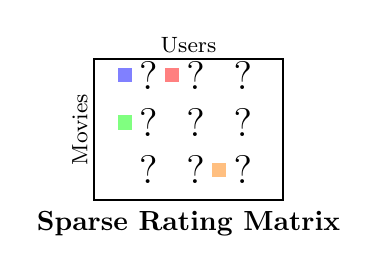
\begin{tikzpicture}[scale=0.6]
    \draw[thick] (0,0) rectangle (4,3);
    \node at (2,3.3) {\footnotesize Users};
    \node[rotate=90] at (-0.3,1.5) {\footnotesize Movies};
    
    % Some filled squares (known ratings)
    \fill[blue!50] (0.5,2.5) rectangle (0.8,2.8);
    \fill[red!50] (1.5,2.5) rectangle (1.8,2.8);
    \fill[green!50] (0.5,1.5) rectangle (0.8,1.8);
    \fill[orange!50] (2.5,0.5) rectangle (2.8,0.8);
    
    % Question marks for missing
    \node at (1.15,2.65) {\Large ?};
    \node at (2.15,2.65) {\Large ?};
    \node at (3.15,2.65) {\Large ?};
    \node at (1.15,1.65) {\Large ?};
    \node at (2.15,1.65) {\Large ?};
    \node at (3.15,1.65) {\Large ?};
    \node at (1.15,0.65) {\Large ?};
    \node at (2.15,0.65) {\Large ?};
    \node at (3.15,0.65) {\Large ?};
    
    \node at (2,-0.5) {\textbf{Sparse Rating Matrix}};
\end{tikzpicture}
\end{center}
}
\end{column}
\end{columns}
\end{frame}

\begin{frame}\vspace{0.5cm}
\textbf{Answer:} $200 \times 10^6 \times 15 \times 10^3 = 3 \times 10^{12}$ possible ratings!

\pause
But typical users rate only 20-100 movies. What percentage of the matrix is filled?

\pause
\textbf{Answer:} $\frac{100}{15000} = 0.67\%$ - extremely sparse!

\end{popquizbox}
\end{frame}

\begin{frame}\begin{equation*}
\mA = \begin{bmatrix}
a_{11} & ? & a_{13} & ? & \cdots \\
? & a_{22} & ? & a_{24} & \cdots \\
a_{31} & ? & ? & a_{34} & \cdots \\
\vdots & \vdots & \vdots & \vdots & \ddots
\end{bmatrix}
\end{equation*}

\pause
\begin{itemize}
\item \textbf{Rows}: Users $u_1, u_2, \ldots, u_N$ 
    \pause
\item \textbf{Columns}: Movies $m_1, m_2, \ldots, m_M$
    \pause
\item \textbf{Entries}: $a_{ij} \in \{1,2,3,4,5\}$ (when observed)
    \pause
\item \textbf{Challenge}: Predict missing entries $?$
    \pause
\item \textbf{Notation}: $\Omega = \{(i,j) : a_{ij} \text{ is observed}\}$
\end{itemize}
\end{frame}

\begin{frame}\begin{center}
\renewcommand{\arraystretch}{1.2}
\begin{tabular}{l|ccccc}
\toprule
\textbf{User} & \textbf{Sholay} & \textbf{Swades} & \textbf{Batman} & \textbf{Interstellar} & \textbf{Shawshank} \\
\midrule
Alice & \textcolor{blue}{5} & \textcolor{blue}{4} & \textcolor{red}{2} & \textcolor{red}{3} & \textcolor{red}{2} \\
Bob & \textcolor{red}{?} & \textcolor{blue}{5} & \textcolor{red}{1} & \textcolor{blue}{4} & \textcolor{red}{?} \\
Carol & \textcolor{blue}{4} & \textcolor{red}{?} & \textcolor{red}{1} & \textcolor{blue}{5} & \textcolor{red}{?} \\
\bottomrule
\end{tabular}
\end{center}

\pause
\textbf{Observations:}
\begin{itemize}
\item Alice loves Bollywood films (Sholay, Swades)
    \item Carol enjoys Sci-Fi (Interstellar)  
    \pause
\item Can we predict Bob's rating for Sholay?
    \item Can we predict Carol's rating for Swades?
\end{itemize}
\end{frame}

\section{Key Insight: Latent Features}

\begin{frame}\begin{columns}[T]
\begin{column}{0.5\textwidth}
\textbf{Maybe because of:}
\begin{itemize}
\item Genre (Action, Romance, Comedy)
    \item Star cast (Shah Rukh Khan, Tom Cruise)
    \pause
\item Director (Christopher Nolan, Rajkumar Hirani)
    \item Language (Hindi, English, Tamil)
    \item Era (90s classics, modern CGI)
\end{itemize}
\end{column}
\begin{column}{0.5\textwidth}
\only<6->{
\textbf{Key Insight:}
\begin{itemize}
\item Your taste = combination of preferences
    \item Movie appeal = combination of features
    \pause
\item \textcolor{red}{But we don't know these explicitly!}
\end{itemize}
}
\end{column}
\end{columns}
\end{frame}

\begin{frame}\textbf{Intuition:} Think of latent features as ``hidden DNA'' of movies and users!

\pause
\vspace{0.5cm}
\textbf{For Movies:}
\begin{itemize}
\item Bollywood vs Hollywood
    \item Action vs Drama  
    \pause
\item Comedy vs Serious
    \item Runtime (Short vs Long)
    \item Year (Classic vs Modern)
\end{itemize}
\end{column}
\begin{column}{0.4\textwidth}
\only<6->{
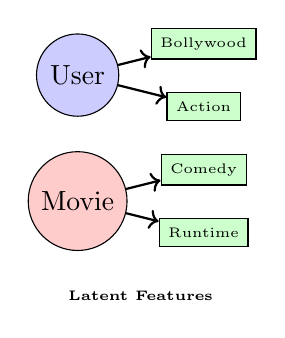
\begin{tikzpicture}[scale=0.8]
    \node[draw, circle, fill=blue!20] (user) at (0,2) {User};
    \node[draw, circle, fill=red!20] (movie) at (0,0) {Movie};
    
    \node[draw, rectangle, fill=green!20] (f1) at (2,2.5) {\tiny Bollywood};
    \node[draw, rectangle, fill=green!20] (f2) at (2,1.5) {\tiny Action};
    \node[draw, rectangle, fill=green!20] (f3) at (2,0.5) {\tiny Comedy};
    \node[draw, rectangle, fill=green!20] (f4) at (2,-0.5) {\tiny Runtime};
    
    \draw[->, thick] (user) -- (f1);
    \draw[->, thick] (user) -- (f2);
    \draw[->, thick] (movie) -- (f3);
    \draw[->, thick] (movie) -- (f4);
    
    \node at (1,-1.5) {\tiny \textbf{Latent Features}};
\end{tikzpicture}
}
\end{column}
\end{columns}
\end{frame}

\begin{frame}\begin{center}
\renewcommand{\arraystretch}{1.3}
\begin{tabular}{l|ccc}
\toprule
\textbf{Movie} & \textbf{Bollywood} & \textbf{Sci-Fi} & \textbf{Drama} \\
\midrule
Sholay & \textcolor{blue}{0.95} & \textcolor{red}{0.10} & \textcolor{orange}{0.85} \\
Swades & \textcolor{blue}{1.00} & \textcolor{red}{0.20} & \textcolor{orange}{0.90} \\
Batman & \textcolor{blue}{0.05} & \textcolor{red}{0.80} & \textcolor{orange}{0.30} \\
Interstellar & \textcolor{blue}{0.05} & \textcolor{red}{0.95} & \textcolor{orange}{0.70} \\
Shawshank & \textcolor{blue}{0.05} & \textcolor{red}{0.15} & \textcolor{orange}{0.95} \\
\bottomrule
\end{tabular}
\end{center}

\pause
\textbf{Movie Feature Matrix} $\mH \in \Real^{3 \times 5}$:
\begin{equation*}
\mH = \begin{bmatrix}
\textcolor{blue}{0.95} & \textcolor{blue}{1.00} & \textcolor{blue}{0.05} & \textcolor{blue}{0.05} & \textcolor{blue}{0.05} \\
\textcolor{red}{0.10} & \textcolor{red}{0.20} & \textcolor{red}{0.80} & \textcolor{red}{0.95} & \textcolor{red}{0.15} \\
\textcolor{orange}{0.85} & \textcolor{orange}{0.90} & \textcolor{orange}{0.30} & \textcolor{orange}{0.70} & \textcolor{orange}{0.95}
\end{bmatrix}
\end{equation*}
\end{frame}

\begin{frame}\begin{equation*}
\mW = \begin{bmatrix}
w_{11} & w_{12} & w_{13} \\
w_{21} & w_{22} & w_{23} \\
w_{31} & w_{32} & w_{33}
\end{bmatrix}
\end{equation*}

\pause
Where row $i$ represents user $i$'s affinity for:
\begin{itemize}
\item $w_{i1}$: Bollywood preference
    \item $w_{i2}$: Sci-Fi preference  
    \pause
\item $w_{i3}$: Drama preference
\end{itemize}

\pause
\textbf{Key Question:} How do we learn these $w_{ij}$ values from observed ratings?
\end{frame}

\begin{frame}\begin{equation*}
\boxed{a_{ij} \approx \vw_i^T \vh_j = \sum_{k=1}^r w_{ik} h_{kj}}
\end{equation*}

\pause
\textbf{In Matrix Form:}
\begin{equation*}
\boxed{\mA \approx \mW \mH}
\end{equation*}

\pause
\begin{center}
$\mA_{3 \times 5} =
\begin{bmatrix}
5 & 4 & 2 & 3 & 2 \\
? & 5 & 1 & 4 & ? \\
4 & ? & 1 & 5 & ? 
\end{bmatrix}
\approx
\begin{bmatrix}
w_{11} & w_{12} & w_{13} \\
w_{21} & w_{22} & w_{23} \\
w_{31} & w_{32} & w_{33}
\end{bmatrix}
\begin{bmatrix}
0.95 & 1.00 & 0.05 & 0.05 & 0.05 \\
0.10 & 0.20 & 0.80 & 0.95 & 0.15 \\
0.85 & 0.90 & 0.30 & 0.70 & 0.95
\end{bmatrix}
= \mW_{3 \times 3} \mH_{3 \times 5}$
\end{center}
\end{frame}

\begin{frame}\begin{columns}[T]
\begin{column}{0.5\textwidth}
\textbf{Alice's Profile:}
\begin{itemize}
\item How much does she like Bollywood? $w_{11}$
    \item How much does she like Action? $w_{12}$
    \pause
\item How much does she like Comedy? $w_{13}$
\end{itemize}
\end{column}
\begin{column}{0.5\textwidth}
\only<4->{
\textbf{Sholay's DNA:}
\begin{itemize}
\item Bollywood-ness: 0.95 (very high!)
    \item Action-ness: 0.10 (low)
    \pause
\item Comedy-ness: 0.85 (high)
\end{itemize}
}
\end{column}
\end{columns}

\pause
\vspace{0.5cm}
\textbf{The Magic Formula:} 
$$\text{Alice's rating} = \text{Alice's preferences} \cdot \text{Sholay's features}$$
\end{frame}

\begin{frame}\textbf{Alice's preferences:} $\vw_1 = [w_{11}, w_{12}, w_{13}]$
\textbf{Sholay's features:} $\vh_1 = [0.95, 0.10, 0.85]^T$

\pause
\begin{align}
\hat{a}_{11} &= \vw_1^T \vh_1 \\
&= w_{11} \cdot 0.95 + w_{12} \cdot 0.10 + w_{13} \cdot 0.85
\end{align}

\pause
\textbf{Goal:} Find $w_{11}, w_{12}, w_{13}$ such that $\hat{a}_{11} \approx 5$ (Alice's actual rating)
\end{frame}

\begin{frame}\begin{enumerate}[<+->]
    \item What are the dimensions of $\mA$? 
    \item What are the dimensions of $\mW$?
    \item What are the dimensions of $\mH$?
    \item How many parameters do we need to learn?
\end{enumerate}

\pause
\textbf{Answers:}
\begin{enumerate}
    \item $\mA \in \Real^{N \times M}$
    \item $\mW \in \Real^{N \times r}$ 
    \item $\mH \in \Real^{r \times M}$
    \item Total parameters: $Nr + rM = r(N + M)$
\end{enumerate}

\pause
\textbf{Key Insight:} If $r \ll \min(N,M)$, we have huge parameter reduction!
\end{tcolorbox}
\end{frame}

\section{Learning the Factorization}

\begin{frame}\begin{equation*}
\boxed{\minimize_{\mW,\mH} \sum_{(i,j) \in \Omega} (a_{ij} - \vw_i^T \vh_j)^2}
\end{equation*}

\pause
\textbf{In Matrix Notation:}
\begin{equation*}
\boxed{\minimize_{\mW,\mH} \|P_\Omega(\mA - \mW\mH)\|_F^2}
\end{equation*}

\pause
Where:
\begin{itemize}
\item $P_\Omega(\cdot)$: projection onto observed entries
    \item $\|\cdot\|_F$: Frobenius norm
    \pause
\item $\Omega$: set of observed $(i,j)$ pairs
\end{itemize}
\end{frame}

\begin{frame}\textbf{Key Insight:} While non-convex jointly, it's convex in each matrix individually!
\end{frame}

\section{Algorithm 1: Alternating Least Squares (ALS)}

\begin{frame}\begin{enumerate}[<+->]
    \item \textbf{Initialize:} $\mW^{(0)}$ and $\mH^{(0)}$ randomly
    \item \textbf{Repeat until convergence:}
    \begin{enumerate}
        \item \textbf{Fix $\mH$, solve for $\mW$:} Each row independently
        \item \textbf{Fix $\mW$, solve for $\mH$:} Each column independently  
    \end{enumerate}
    \item Each subproblem is a standard least squares problem!
\end{enumerate}

\pause
\begin{center}
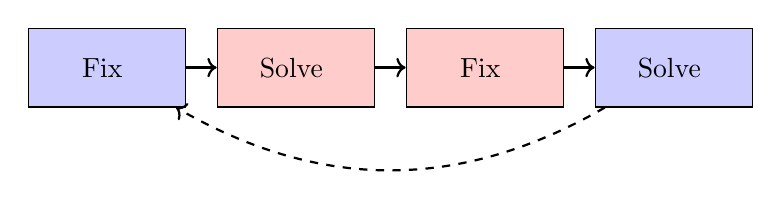
\begin{tikzpicture}[scale=0.8]
    \node[draw, fill=blue!20, minimum width=2cm, minimum height=1cm] (W) at (0,0) {Fix $\mW$};
    \node[draw, fill=red!20, minimum width=2cm, minimum height=1cm] (H) at (3,0) {Solve $\mH$};
    \node[draw, fill=red!20, minimum width=2cm, minimum height=1cm] (W2) at (6,0) {Fix $\mH$};
    \node[draw, fill=blue!20, minimum width=2cm, minimum height=1cm] (H2) at (9,0) {Solve $\mW$};
    
    \draw[->, thick] (W) -- (H);
    \draw[->, thick] (H) -- (W2);
    \draw[->, thick] (W2) -- (H2);
    \draw[->, thick, dashed] (H2) to[bend left] (W);
\end{tikzpicture}
\end{center}
\end{frame}

\begin{frame}\begin{equation*}
\minimize_{\vw_i} \sum_{j: (i,j) \in \Omega} (a_{ij} - \vw_i^T \vh_j)^2
\end{equation*}

\pause
\textbf{Matrix Form for User $i$:}
Let $\Omega_i = \{j: (i,j) \in \Omega\}$ (movies rated by user $i$)

\pause
\begin{align}
\vy_i &= [a_{i,j_1}, a_{i,j_2}, \ldots, a_{i,j_{|\Omega_i|}}]^T \\
\mX_i &= [\vh_{j_1}, \vh_{j_2}, \ldots, \vh_{j_{|\Omega_i|}}]^T
\end{align}

\pause
\textbf{Least Squares Solution:}
\begin{equation*}
\boxed{\vw_i^* = (\mX_i^T \mX_i)^{-1} \mX_i^T \vy_i}
\end{equation*}
\end{frame}

\begin{frame}\begin{align}
\vy_1 &= \begin{bmatrix} 5 \\ 4 \\ 2 \\ 3 \\ 2 \end{bmatrix} \\
\mX_1 &= \begin{bmatrix} 
0.95 & 0.10 & 0.85 \\
1.00 & 0.20 & 0.90 \\
0.05 & 0.80 & 0.30 \\
0.05 & 0.95 & 0.70 \\
0.05 & 0.15 & 0.95
\end{bmatrix}
\end{align}

\pause
\textbf{Solution:} $\vw_1^* = (\mX_1^T \mX_1)^{-1} \mX_1^T \vy_1$

This gives us Alice's feature preferences!
\end{frame}

\begin{frame}\begin{equation*}
\minimize_{\vh_j} \sum_{i: (i,j) \in \Omega} (a_{ij} - \vw_i^T \vh_j)^2
\end{equation*}

\pause
\textbf{Matrix Form for Movie $j$:}
Let $\Omega_j = \{i: (i,j) \in \Omega\}$ (users who rated movie $j$)

\pause
\begin{align}
\vy_j &= [a_{i_1,j}, a_{i_2,j}, \ldots, a_{i_{|\Omega_j|},j}]^T \\
\mX_j &= [\vw_{i_1}, \vw_{i_2}, \ldots, \vw_{i_{|\Omega_j|}}]^T
\end{align}

\pause
\textbf{Least Squares Solution:}
\begin{equation*}
\boxed{\vh_j^* = (\mX_j^T \mX_j)^{-1} \mX_j^T \vy_j}
\end{equation*}
\end{frame}

\begin{frame}\textbf{Objective Function:}
\begin{equation*}
L(\mW, \mH) = \sum_{(i,j) \in \Omega} (a_{ij} - \vw_i^T \vh_j)^2
\end{equation*}

\pause
\textbf{Gradients:}
\begin{align}
\frac{\partial L}{\partial \vw_i} &= -2 \sum_{j: (i,j) \in \Omega} (a_{ij} - \vw_i^T \vh_j) \vh_j \\
\frac{\partial L}{\partial \vh_j} &= -2 \sum_{i: (i,j) \in \Omega} (a_{ij} - \vw_i^T \vh_j) \vw_i
\end{align}
\end{frame}

\begin{frame}\begin{columns}[T]
\begin{column}{0.5\textwidth}
\textbf{Your Process:}
\begin{enumerate}[<+->]
    \item Make a guess about their rating
    \item See their actual rating
    \item Adjust your understanding
    \item Repeat for next movie
\end{enumerate}
\end{column}
\begin{column}{0.5\textwidth}
\only<5->{
\textbf{SGD does exactly this!}
\begin{itemize}
\item One rating at a time
    \item Small adjustments
    \pause
\item Gradually improves
\end{itemize}
}
\end{column}
\end{columns}
\end{frame}

\begin{frame}\begin{enumerate}[<+->]
    \item \textbf{Predict:} $\hat{a}_{ij} = \vw_i^T \vh_j$
    \item \textbf{Compute Error:} $e_{ij} = a_{ij} - \hat{a}_{ij}$  
    \item \textbf{Update:}
    \begin{align}
    \vw_i &\leftarrow \vw_i + \alpha \cdot e_{ij} \cdot \vh_j \\
    \vh_j &\leftarrow \vh_j + \alpha \cdot e_{ij} \cdot \vw_i
    \end{align}
\end{enumerate}

\pause
\textbf{Intuition:}
\begin{itemize}
\item If $e_{ij} > 0$: Predicted rating too low → Increase similarity
    \item If $e_{ij} < 0$: Predicted rating too high → Decrease similarity
    \pause
\item Learning rate $\alpha$ controls step size
\end{itemize}
\end{frame}

\begin{frame}\begin{align}
\text{Current: } &\vw_1 = [0.4, 0.2, 0.3], \quad \vh_1 = [0.95, 0.10, 0.85] \\
\text{Prediction: } &\hat{a}_{11} = 0.4 \times 0.95 + 0.2 \times 0.10 + 0.3 \times 0.85 = 0.655 \\
\text{Error: } &e_{11} = 5 - 0.655 = 4.345
\end{align}

\pause
\textbf{Updates with $\alpha = 0.01$:}
\begin{align}
\vw_1 &\leftarrow [0.4, 0.2, 0.3] + 0.01 \times 4.345 \times [0.95, 0.10, 0.85] \\
&= [0.4413, 0.2043, 0.3369] \\
\vh_1 &\leftarrow [0.95, 0.10, 0.85] + 0.01 \times 4.345 \times [0.4, 0.2, 0.3] \\
&= [0.9674, 0.1087, 0.8631]
\end{align}
\end{frame}

\begin{frame}\begin{enumerate}[<+->]
    \item What is the error $e_{ij}$?
    \item Should we increase or decrease the user-movie similarity?
    \item If $\alpha = 0.1$, $\vw_i = [0.8, 0.3]$, $\vh_j = [0.6, 0.9]$, what are the updates?
\end{enumerate}

\pause
\textbf{Answers:}
\begin{enumerate}
    \item $e_{ij} = 2 - 4.5 = -2.5$
    \item Decrease similarity (negative error)
    \item $\vw_i \leftarrow [0.8, 0.3] + 0.1 \times (-2.5) \times [0.6, 0.9] = [0.65, 0.075]$
    \item $\vh_j \leftarrow [0.6, 0.9] + 0.1 \times (-2.5) \times [0.8, 0.3] = [0.4, 0.825]$
\end{enumerate}
\end{tcolorbox}
\end{frame}

\section{Algorithm Comparison and Practical Considerations}

\begin{frame}\textbf{When to Use Which?}
\begin{itemize}
\item \textbf{ALS:} Large-scale, production systems (Spark, distributed)
    \pause
\item \textbf{SGD:} Online learning, real-time updates, research
\end{itemize}
\end{frame}

\begin{frame}\textbf{Bias Terms:} Account for global, user, and item biases
\begin{equation*}
\hat{a}_{ij} = \mu + b_i + b_j + \vw_i^T \vh_j
\end{equation*}

\pause
\textbf{Implicit Feedback:} Binary observations (clicks, views)
\begin{equation*}
\text{Confidence: } c_{ij} = 1 + \alpha \cdot \text{frequency}_{ij}
\end{equation*}

\pause
\textbf{Cold Start Problem:} New users/items with no ratings
\begin{itemize}
\item Content-based features
    \item Demographic information  
    \pause
\item Hybrid approaches
\end{itemize}
\end{frame}

\section{Hands-On Understanding}

\begin{frame}\textbf{Goal:} Find $\mW \in \Real^{3 \times 2}$ and $\mH \in \Real^{2 \times 3}$ such that:
\begin{equation*}
\mA \approx \mW \mH = \begin{bmatrix}
w_{11} & w_{12} \\
w_{21} & w_{22} \\
w_{31} & w_{32}
\end{bmatrix}
\begin{bmatrix}
h_{11} & h_{12} & h_{13} \\
h_{21} & h_{22} & h_{23}
\end{bmatrix}
\end{equation*}

\pause
\textbf{Constraint:} Only minimize error on observed entries!
\end{frame}

\begin{frame}\textbf{Update User 1:} Only use observed ratings (positions 1,3)
\begin{align}
\vy_1 &= [5, 2]^T \\
\mX_1 &= \begin{bmatrix} 1.0 & 0.3 \\ 0.2 & 0.8 \end{bmatrix} \text{ (columns 1,3 of } \mH^{(0)T}\text{)}
\end{align}

\pause
\textbf{Solve:} $\vw_1^{(1)} = (\mX_1^T \mX_1)^{-1} \mX_1^T \vy_1$

Continue for all users and movies...
\end{frame}

\begin{frame}Design your recommendation system:
\begin{enumerate}[<+->]
    \item Which algorithm: ALS or SGD? Why?
    \item What rank $r$ would you choose?
    \item How to handle new users?
    \item How to handle the scale?
\end{enumerate}

\pause
\textbf{Suggested Solution:}
\begin{itemize}
\item \textbf{ALS} for batch processing (Spark), \textbf{SGD} for online updates
    \item $r = 50-200$ (balance between expressiveness and efficiency)
    \pause
\item Hybrid: Content-based for cold start + collaborative filtering
    \item Distributed computing, approximate algorithms, caching
\end{itemize}
\end{tcolorbox}
\end{frame}

\section{Summary and Key Takeaways}

\begin{frame}\textbf{The Mathematical Beauty:}
\begin{equation*}
\boxed{\text{Collaborative Filtering} = \text{Matrix Factorization} = \text{Dimensionality Reduction}}
\end{equation*}
\end{frame}

\begin{frame}\begin{itemize}
\item \textbf{Non-negative Matrix Factorization (NMF)}: Interpretable factors
    
    \pause
\item \textbf{Deep Matrix Factorization}: Neural networks for non-linear patterns
    
    \pause
\item \textbf{Factorization Machines}: Handle multi-way interactions
    
    \pause
\item \textbf{Variational Autoencoders}: Probabilistic approach to recommendations
    
    \pause
\item \textbf{Graph Neural Networks}: Leverage user-item interaction graphs
    
    \pause
\item \textbf{Multi-armed Bandits}: Exploration vs exploitation in recommendations
\end{itemize}

\pause
\textbf{Applications Beyond Movies:}
\begin{itemize}
\item E-commerce (Amazon, eBay)
    \item Music streaming (Spotify, Apple Music)  
    \pause
\item Social media (Facebook, LinkedIn)
    \item Online advertising (Google, Facebook)
\end{itemize}
\end{frame}

\begin{frame}\begin{enumerate}[<+->]
    \item Matrix factorization can only work with explicit ratings
    \item ALS always converges to the global optimum  
    \item A rank-1 factorization means all users have identical preferences
    \item Adding regularization always improves recommendations
    \item SGD is better than ALS for all applications
\end{enumerate}

\pause
\textbf{Answers:}
\begin{enumerate}
    \item \textbf{False} - Works with implicit feedback too (clicks, views)
    \item \textbf{False} - Converges to local optimum (problem is non-convex)
    \item \textbf{False} - Rank-1 means one dominant pattern, not identical preferences
    \item \textbf{False} - Too much regularization can cause underfitting
    \item \textbf{False} - Choice depends on scale, parallelization needs, stability requirements
\end{enumerate}
\end{tcolorbox}
\end{frame}

\begin{frame}[standout]
\Huge \textbf{Questions?}
\vspace{1em}

\Large Thank you for your attention!
\vspace{1em}

\normalsize
Next: Deep learning approaches to recommendation systems
\end{frame}

\end{document}